% Alternate illustrated wrap; spine typography matches the original.
% KDP wrap. bin/kdp-cover supplies dimensions from the
% finished interior PDF, so pagination changes cannot stale the spine.
\documentclass{article}
\input{\CoverDimensionsFile}
\usepackage[paperwidth=\CoverSheetWidth,paperheight=\CoverSheetHeight,margin=0pt]{geometry}
\usepackage{graphicx}
\usepackage[cmyk]{xcolor}
\usepackage{tikz}
\usepackage{fontspec}
\usepackage{adjustbox}
\pagestyle{empty}

%\definecolor{CoverBackground}{cmyk}{0.23,0.10,0.00,0.77}
\definecolor{CoverBackground}{cmyk}{0.22,0.10,0.00,0.88}
\definecolor{CoverForeground}{cmyk}{0.00,0.03,0.09,0.09}

% KDP requires every spine-text edge to stay 0.0625 in inside the folds.
\newcommand{\SpineLabel}[2]{%
  \adjustbox{max width=\dimexpr\CoverSpineWidth-0.125in\relax}{\fontsize{#1}{#1}\selectfont #2}%
}
% Shared geometric LD mark.  Keep the artwork independent of font metrics and
% leave its color unset so it inherits the surrounding text/TikZ color.
%
% Usage: \LD, \LD[height], or \LD[height][width].  Width defaults to 90% of
% height; giving it explicitly makes the mark's aspect ratio independently
% adjustable without changing its geometry.
\ProvideDocumentCommand{\LD}{O{1em} o}{%
  \IfNoValueTF{#2}
    {\pgfmathsetlengthmacro{\LDWidth}{0.9*(#1)}}
    {\pgfmathsetlengthmacro{\LDWidth}{#2}}%
  \tikz[baseline=0pt,x=\LDWidth,y=#1]{%
    % The normalized 1 x 1 box includes a narrow optical margin.  Each
    % component is the same square-cornered L, with the second rotated by
    % 180 degrees.
    \path[use as bounding box] (0,0) rectangle (1,1);
    \fill
      (0.04,0.04) rectangle (0.18,0.96)
      (0.04,0.04) rectangle (0.69,0.18)
      (0.82,0.04) rectangle (0.96,0.96)
      (0.31,0.82) rectangle (0.96,0.96);
  }%
}

\def\CoverSpineLD{ld}
\newcommand{\SpineName}{%
  \ifx\CoverSpine\CoverSpineLD
    % Keep the mark about as tall as the front-cover "The Nameless", but use
    % the taller 50:64 proportions requested for the spine.
    \SpineLabel{22}{\LD[1em][0.78em]}%
  \else
    \SpineLabel{15}{\shortstack{The\\Nameless}}%
  \fi
}

\ifdefined\CoverShowSpine\else\def\CoverShowSpine{true}\fi
\def\CoverShowSpineTrue{true}
\newsavebox{\CoverInkBox}
\newcommand{\CenterCoverInk}[1]{%
  \sbox{\CoverInkBox}{#1}%
  \raisebox{\dimexpr(\dp\CoverInkBox-\ht\CoverInkBox)/2\relax}{\usebox{\CoverInkBox}}%
}
\begin{document}
\begin{tikzpicture}[remember picture,overlay,x=1in,y=1in]
  \ifdefined\CoverIllustrated
    % Extend artwork through turn-ins; keep the framed panels out of the hinges.
% Source PNGs are prepared once, never regenerated during a publication build.
\node[inner sep=0pt] at (current page.center)
  {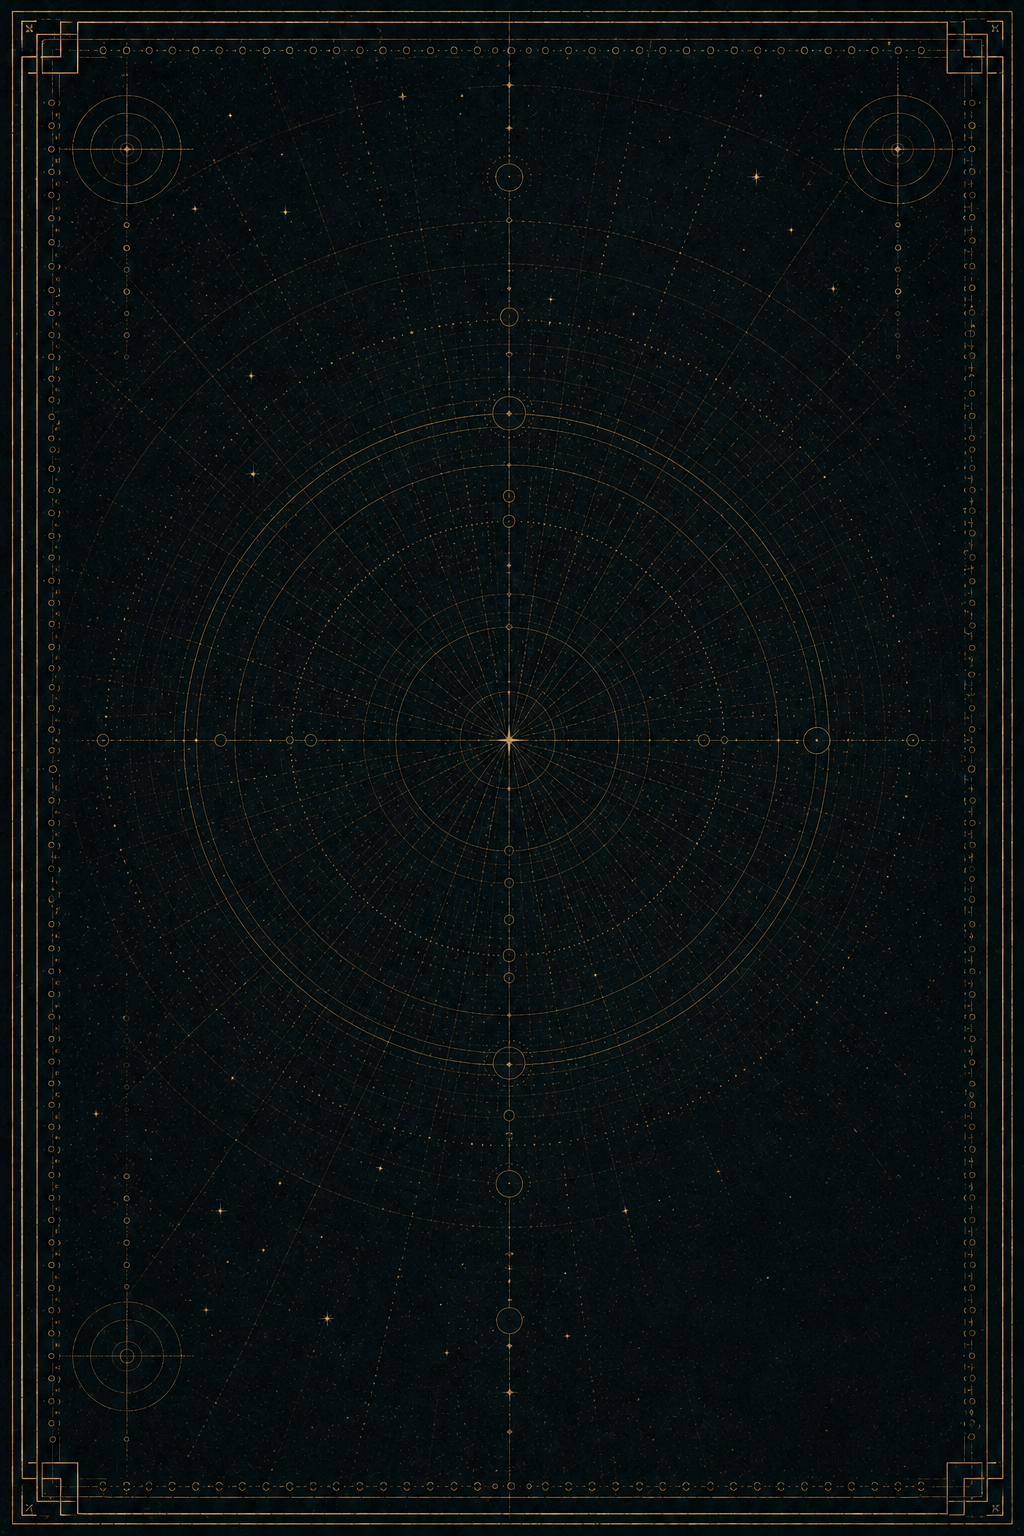
\includegraphics[width=\CoverSheetWidth,height=\CoverSheetHeight]{pub/covers/fancy/assets/back.png}};
% Engraving continues through the spine, hinges, and turn-ins.
\begin{scope}
  \clip ([xshift=\dimexpr\CoverBleed+\CoverPanelWidth\relax]current page.south west)
    rectangle ([xshift=\CoverFrontLeft]current page.north west);
  \node[inner sep=0pt] at (current page.center)
    {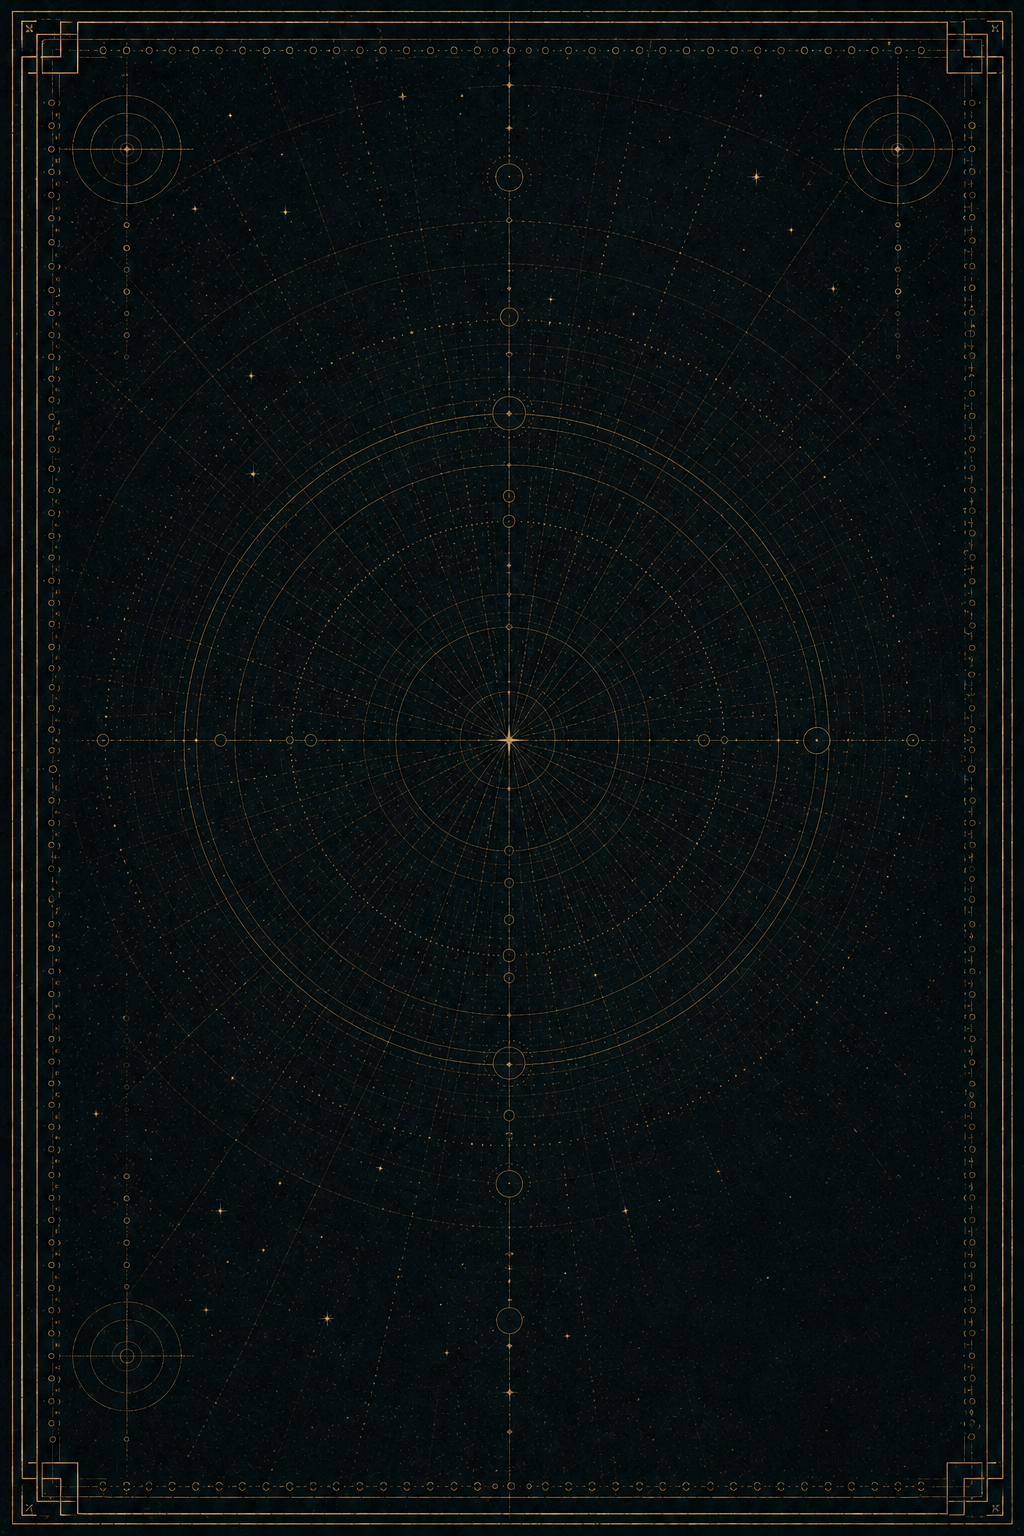
\includegraphics[height=\CoverSheetHeight]{pub/covers/fancy/assets/back.png}};
\end{scope}
\foreach \side/\image in {west/back,east/front-textless} {
  \begin{scope}
    \def\WestSide{west}
    \ifx\side\WestSide
      \coordinate (panelCenter) at ([xshift=\dimexpr\CoverBleed+\CoverPanelWidth/2\relax]current page.west);
    \else
      \coordinate (panelCenter) at ([xshift=-\dimexpr\CoverBleed+\CoverPanelWidth/2\relax]current page.east);
    \fi
    \clip ([xshift=-\CoverPanelWidth/2,yshift=-\CoverPanelHeight/2]panelCenter)
      rectangle ([xshift=\CoverPanelWidth/2,yshift=\CoverPanelHeight/2]panelCenter);
    \node[inner sep=0pt] at (panelCenter)
      {\includegraphics[width=\CoverPanelWidth,height=\CoverPanelHeight]{pub/covers/fancy/assets/\image.png}};
  \end{scope}
}

  \else
  \fill[CoverBackground] (current page.south west) rectangle (current page.north east);

  \fi
  \coordinate (frontSW) at
    ([xshift=\CoverFrontLeft,yshift=\CoverBleed]current page.south west);
  % Artwork coordinates measured in front-textless.png (1024 x 1536).
  % Use ink centers, including descenders in arbitrary sub-book titles.
  \coordinate (circleCenter) at
    ([xshift=0.497\CoverPanelWidth,yshift=0.518\CoverPanelHeight]frontSW);
  % Share these ink-center heights with the spine; all tuning happens here.
  \coordinate (coverWe) at
    ([yshift=\CoverTitleSeparation\CoverPanelHeight]circleCenter);
  \coordinate (coverNameless) at
    ([yshift=-\CoverTitleSeparation\CoverPanelHeight]circleCenter);
  \coordinate (coverVolume) at
    ([yshift=-\CoverVolumeOffset\CoverPanelHeight]circleCenter);
  \coordinate (spineAxis) at
    ([xshift=\CoverSpineCenterX]current page.south west);
  \node[CoverForeground,anchor=base,inner sep=0pt] at
    (coverWe)
    {\CenterCoverInk{\fontsize{100}{120}\selectfont\textsc{We}}};
  \node[CoverForeground,anchor=base,inner sep=0pt] at (coverNameless)
    {\CenterCoverInk{\fontsize{25}{30}\selectfont The Nameless}};
  \node[CoverForeground,anchor=base,inner sep=0pt] at
    (coverVolume)
    {\CenterCoverInk{\fontsize{23}{28}\selectfont \CoverVolume}};

  \ifx\CoverShowSpine\CoverShowSpineTrue
  \node[CoverForeground,anchor=base,inner sep=0pt] at
    (spineAxis |- coverWe)
    {\CenterCoverInk{\SpineLabel{26}{\textsc{We}}}};
  \node[CoverForeground,anchor=base,inner sep=0pt,align=center] at
    (spineAxis |- coverNameless)
    {\CenterCoverInk{\SpineName}};
  \node[CoverForeground,anchor=base,inner sep=0pt] at
    (spineAxis |- coverVolume)
    {\CenterCoverInk{\SpineLabel{18}{\CoverVolume}}};
  \fi
\end{tikzpicture}
\null
\end{document}
